%!TEX root = edance.tex
%%%%%%%%%%%%%%%%
%   CHAPTER 7  %
%%%%%%%%%%%%%%%%
\chapter{MOS Capacitor}
\label{ch:ch07_mos_c}
\graphicspath{{./figs_MOS_C/}}
%%%%%%%%%%%%%%%%%%%%%%%%%%%%%%%%%%%%%%%%%%%%%%%%%%%%%%%%%%%%%%%%%%%%%%%%%%%%%%%%%%%%%%%%
%%%%%%%%%%%%%%%%%%%%%%%%%%%%%%%%%%%%%%%%%%%%%%%%%%%%%%%%%%%%%%%%%%%%%%%%%%%%%%%%%%%%%%%%
%                                   SECTION 7.1                                        %
%%%%%%%%%%%%%%%%%%%%%%%%%%%%%%%%%%%%%%%%%%%%%%%%%%%%%%%%%%%%%%%%%%%%%%%%%%%%%%%%%%%%%%%%
%%%%%%%%%%%%%%%%%%%%%%%%%%%%%%%%%%%%%%%%%%%%%%%%%%%%%%%%%%%%%%%%%%%%%%%%%%%%%%%%%%%%%%%%
\section{Chapter Preview}
In this chapter we will be learning about the Metal-Oxide-Silicon (MOS) capacitor (MOS-C) structure (see \emph{Fig.~\ref{fig:mos_cap}}). Like most capacitors, it has two plates separated by an insulator.  One plate, the "gate", is nominally made of either a metal, or a heavily doped semiconductor that for all intents and purposes acts like a metal.  The other plate, the "body",  is made of a semiconductor like silicon, and this makes the behavior very different from a regular (metal-insulator-metal) capacitor. It is important to understand this behavior in detail, and the different modes of operations in a MOS-C.  We shall find that the MOS-C structure behaves very much like a $PN$-junction in the that it has a built-in potential and a depletion region.  This causes the capacitor to have built-in charge, even with zero bias and a thicker effective insulator in certain regions of operation.  We will also demonstrate that there is a threshold voltage that, if exceeded, causes the bottom plate surface to "invert" from one type of semiconductor to the opposite kind.  When the surface of the bottom plate reaches this inversion state, a conducting charge sheet is formed that acts like the second plate.  The threshold voltage is extremely important when we discuss MOS transistors in the next chapter, because this charge sheet will be the channel for current conduction.  We will also investigate the fields and potentials in various parts of the device in the various regions of operation.  We will conclude the chapter by discussing the quantitative $Q$-$V$ and $C$-$V$ curves.
\newpage
%%%%%%%%%%%%%%%%%%%%%%%%%%%%%%%%%%%%%%%%%%%%
%                 FIGURE                   %
%%%%%%%%%%%%%%%%%%%%%%%%%%%%%%%%%%%%%%%%%%%%
\begin{figure}[t]
\centering
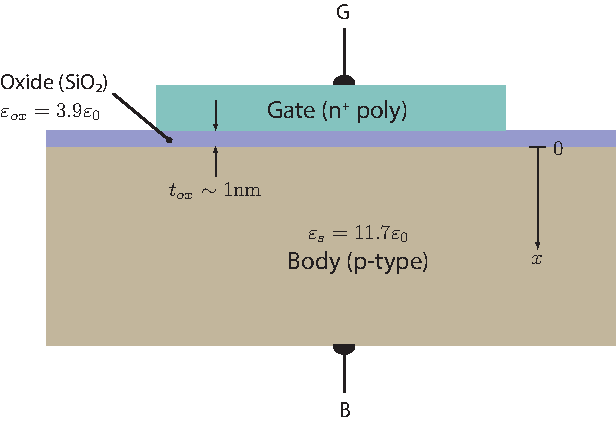
\includegraphics[width=\columnwidth]{mos_cap_structure}
\caption{The Metal-Oxide-Semiconductor Capacitor  (MOS-C) structure.  The structure has a "gate" (G) terminal and a "body" (B) terminal.  As shown, it is an NMOS-C realized with an $N$-type polysilicon gate (heavily doped) and a $P$-type body.}
\label{fig:mos_cap}
\end{figure}
%%%%%%%%%%%%%%%%%%%%%%%%%%%%%%%%%%%%%%%%%%%%%%%%%%%%%%%%%%%%%%%%%%%%%%%%%%%%%%%%%%%%%%%%
%%%%%%%%%%%%%%%%%%%%%%%%%%%%%%%%%%%%%%%%%%%%%%%%%%%%%%%%%%%%%%%%%%%%%%%%%%%%%%%%%%%%%%%%
%                                   SECTION 7.2                                        %
%%%%%%%%%%%%%%%%%%%%%%%%%%%%%%%%%%%%%%%%%%%%%%%%%%%%%%%%%%%%%%%%%%%%%%%%%%%%%%%%%%%%%%%%
%%%%%%%%%%%%%%%%%%%%%%%%%%%%%%%%%%%%%%%%%%%%%%%%%%%%%%%%%%%%%%%%%%%%%%%%%%%%%%%%%%%%%%%%
\section{MOS Capacitor Structure}
%%%%%%%%%%%%%%%%%%%%%%%%%%%%%%%%%%%%%%%%%%%%
%             SUBSECTION 7.2.1             %
%%%%%%%%%%%%%%%%%%%%%%%%%%%%%%%%%%%%%%%%%%%%
\subsection{MOS Capacitor}
The \textbf{Metal Oxide Semiconductor Capacitor}\index{MOS capacitor} (MOS-C) structure shown in \emph{Fig.~\ref{fig:mos_cap}}, is a sandwich of conductors separated by an insulator.  The device has two terminals, the \textbf{gate}\index{MOS capacitor!gate} and the \textbf{body}\index{MOS capacitor!body}, and a voltage is applied between the gate and body through these terminals.  The  “metal” gate is more commonly a heavily doped polysilicon (poly-$Si$) layer doped $n^+$ or $p^+$.  The gate was originally made of metal (e.g. $Al$) until around 1970, but changed to poly-$Si$ due to high temperature processing.  After 2008, metal gates have been reintroduced for various technical reasons that we will not discuss in this book.  Because the body is a semiconductor, there are two possible flavors of MOS-C devices.  The \textbf{NMOS capacitor}\index{MOS capacitor!NMOS} uses a $P$-type substrate, and the \textbf{PMOS capacitor}\index{MOS capacitor!PMOS} uses an $N$-type substrate.  Note that this is not a typo!  The body doping is opposite to the flavor, something which we will clarify in this chapter.  Finally, the insulator can in theory be any non-conductor, but in practice for silicon MOS structures $SiO_2$ is the oxide of choice.  This is because it is native to $Si$ (easy to grow, very low surface defects), and it can double as a mask opening during fabrication (blocking implants).  Ideally this layer is very thin, with modern devices using a few layers of atoms to realize the lowest thickness possible.  Because there is a physical limit to how thin we can make this layer\footnote{Due to leakage currents through the gate and the fact that a very thin layer can undergo oxide breakdown since even modest gate-to-body voltages impose large electric fields.}, modern devices may use a stack up of layers including higher \textbf{dielectric constant}\index{Capacitor!dielectric constant} (high "K") insulators.  Native $SiO_2$ has a relative permittivity of $3.9$, which is about three times smaller than silicon.
%%%%%%%%%%%%%%%%%%%%%%%%%%%%%%%%%%%%%%%%%%%%
%                 FIGURE                   %
%%%%%%%%%%%%%%%%%%%%%%%%%%%%%%%%%%%%%%%%%%%%
\begin{figure}[t]
\centering
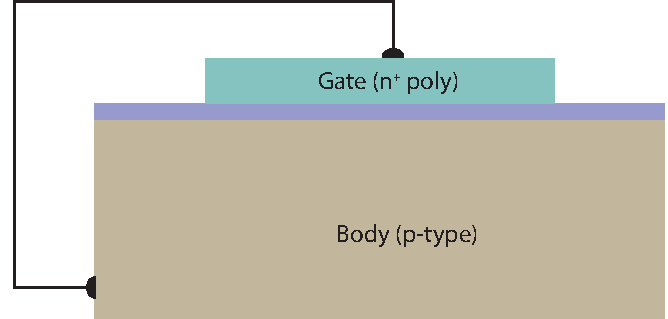
\includegraphics[width=\columnwidth]{mos_cap_wire_short}
\caption{The MOS-C with gate/body shorted in equilibrium. }
\label{fig:mos_cap_gate_body_short}
\end{figure}
%%%%%%%%%%%%%%%%%%%%%%%%%%%%%%%%%%%%%%%%%%%%
%             SUBSECTION 7.2.2             %
%%%%%%%%%%%%%%%%%%%%%%%%%%%%%%%%%%%%%%%%%%%%
\subsection{Metal-Oxide-Semiconductor Junction}
Consider applying zero volts between the gate and the body, or in other words shorting the gate to the body as shown in \emph{Fig.~\ref{fig:mos_cap_gate_body_short}}.  With this connection, we are allowing currents to flow between the gate and body.  In particular, due to diffusion currents\index{Current!diffusion}, we expect many electrons to leave the gate and enter the body. Likewise, holes in the body will naturally diffuse to the gate.  Under thermal equilibrium\index{Thermal equilibrium}, current flow will cease and therefore the $N$-type poly gate will rise to a higher potential than the $P$-type substrate, just like in a $PN$-junction diode.  Using intrinsic silicon as a reference, the potential of the $P$-type region is given by:
    \begin{equation}
        \varphi_p = -\left( \frac{kT}{q} \right) \cdot \ln \left( \frac{N_A}{n_i} \right)
        \label{eq:p_body_pot}
    \end{equation}
The potential of the $N$-type gate is given by:
    \begin{equation}
        \varphi_{poly,{n^+}} = \left( \frac{kT}{q} \right) \cdot \ln \left( {\frac{N_{d,poly}}{n_i}} \right) \approx 550\,mV
        \label{eq:n_gate_pot}
    \end{equation}
Note that the $N$-type gate is heavily doped, so we can approximate the potential as $550\,mV$ if the doping level is not given.  In equilibrium, no current can flow because the insulator blocks DC currents.  But from our knowledge of $PN$-junctions, and with reference to \emph{Eq.~\ref{eq:p_body_pot}} and \emph{Eq.~\ref{eq:n_gate_pot}}, we know the flow of majority carrier diffusion will stop due to the \textbf{built-in potential difference}\index{MOS capacitor!built-in potential difference}:
    \begin{align}
        \Aboxed{ \varphi_{bi} &= \varphi_{poly,{n^+}} - \varphi_p }  &\textit{Built-in potential, NMOS-C}
        \label{eq:built_in_nmos_c}
    \end{align}
This potential difference is accompanied by an electric field and fields terminate on charge.  Where are these fields and charges?
\newpage
%%%%%%%%%%%%%%%%%%%%%%%%%%%%%%%%%%%%%%%%%%%%
%                 FIGURE                   %
%%%%%%%%%%%%%%%%%%%%%%%%%%%%%%%%%%%%%%%%%%%%
\begin{figure}[t]
\centering
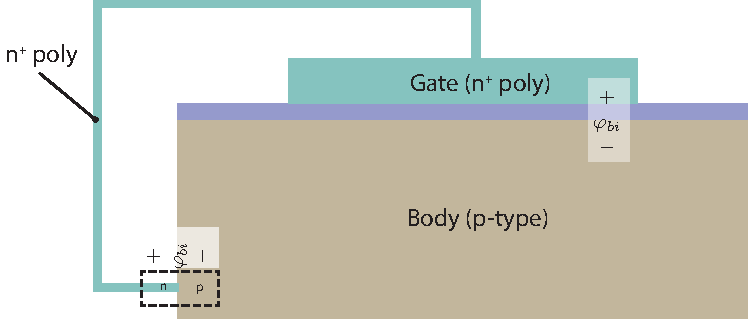
\includegraphics[width=.95\columnwidth]{mos_cap_short_phibi}
\caption{The MOS-C structure with gate-to-body shorted using a polysilicon gate material as the routing wire.  The built-in potential $\varphi_{bi}$ that develops across the $PN$-junction results also in a  potential drop across the oxide.}
\label{fig:mos_cap_gate_body_short_gate}
\end{figure}
%%%%%%%%%%%%%%%%%%%%%%%%%%%%%%%%%%%%%%%%%%%%
%             SUBSECTION 7.2.3             %
%%%%%%%%%%%%%%%%%%%%%%%%%%%%%%%%%%%%%%%%%%%%
\subsection{Gate Materials and Contact Potential}
%%%%%%%%%%%%%%%%%%%%%%%%%%%%%%%%%%%%%%%%%%%%
%              SUB-SUBSECTION              %
%%%%%%%%%%%%%%%%%%%%%%%%%%%%%%%%%%%%%%%%%%%%
\subsubsection{What about contact potentials?}
Technically, so far we have actually been analyzing the structure shown in \emph{Fig.~\ref{fig:mos_cap_gate_body_short_gate}}.  In other words, we have been assuming that the wires connecting the gate to the body are made of the same material as the gate.  There are two built-in potentials that cancel out as we go around the loop. One built-in potential is between the $PN$-junction\index{PN-junction} (the body to poly-$n^+$ wire connection), which is just like any other $PN$-junction that we have studied so far.  The other built-in potential is dropped across the oxide layer between the body and gate.  
%%%%%%%%%%%%%%%%%%%%%%%%%%%%%%%%%%%%%%%%%%%%
%              SUB-SUBSECTION              %
%%%%%%%%%%%%%%%%%%%%%%%%%%%%%%%%%%%%%%%%%%%%
\subsubsection{Real Wires}
In practice, the wire interconnect is not the poly-$n^+$ gate material,\footnote{Poly gate is often used for some of the routing in integrated circuits, but most routing is with metal layers}, but instead a metal like aluminum or copper.  The complete structure is shown in \emph{Fig.~\ref{fig:mos_cap_gate_body_short_wire}}, which shows that there is a $p^+$ region in the body that forms a contact to the body.  Heavily doped diffusion regions form “ohmic” contacts\index{Ohmic contact}, rather than \textbf{rectifying contacts}\index{Rectifying contact}.  Some contact engineering is also required to make the contact between the metal and the gate (not shown). In essence, suitable materials are used to avoid rectifying contacts.  
%%%%%%%%%%%%%%%%%%%%%%%%%%%%%%%%%%%%%%%%%%%%
%                 FIGURE                   %
%%%%%%%%%%%%%%%%%%%%%%%%%%%%%%%%%%%%%%%%%%%%
\begin{figure}[H]
\centering
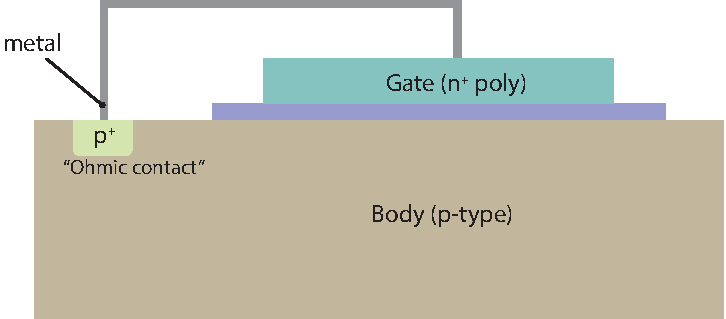
\includegraphics[width=.75\columnwidth]{mos_cap_metal_short}
\caption{In practice, the gate to body connection is made partially with aluminium or copper wires.  Special material selection is required (not shown) to avoid making rectifying contacts between the metal layers and the semiconductors.  A $p^+$ heavily doped region acts as a contact point for the body.} \label{fig:mos_cap_gate_body_short_wire}
\end{figure}
%%%%%%%%%%%%%%%%%%%%%%%%%%%%%%%%%%%%%%%%%%%%
\newpage
%%%%%%%%%%%%%%%%%%%%%%%%%%%%%%%%%%%%%%%%%%%%
%                 FIGURE                   %
%%%%%%%%%%%%%%%%%%%%%%%%%%%%%%%%%%%%%%%%%%%%
\begin{figure}[t]
\centering
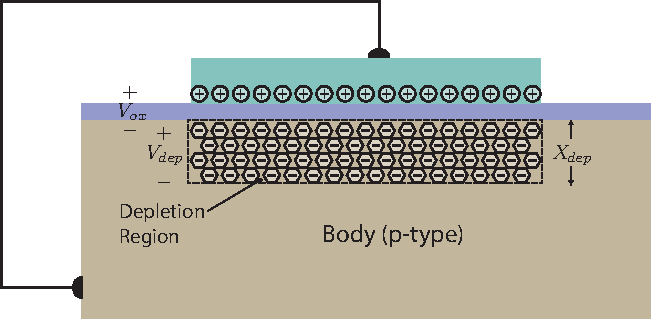
\includegraphics[width=.85\columnwidth]{mos_cap_equilibrium}
\caption{In equilibrium, there is a potential drop across the oxide and the silicon surface (depletion region) corresponding to the built-in potential between the gate and body.}
\label{fig:mos_charge_equil}
\end{figure}
%%%%%%%%%%%%%%%%%%%%%%%%%%%%%%%%%%%%%%%%%%%%%%%%%%%%%%%%%%%%%%%%%%%%%%%%%%%%%%%%%%%%%%%%
%%%%%%%%%%%%%%%%%%%%%%%%%%%%%%%%%%%%%%%%%%%%%%%%%%%%%%%%%%%%%%%%%%%%%%%%%%%%%%%%%%%%%%%%
%                                   SECTION 7.3                                        %
%%%%%%%%%%%%%%%%%%%%%%%%%%%%%%%%%%%%%%%%%%%%%%%%%%%%%%%%%%%%%%%%%%%%%%%%%%%%%%%%%%%%%%%%
%%%%%%%%%%%%%%%%%%%%%%%%%%%%%%%%%%%%%%%%%%%%%%%%%%%%%%%%%%%%%%%%%%%%%%%%%%%%%%%%%%%%%%%%
\section{MOS Regions of Operation}
%%%%%%%%%%%%%%%%%%%%%%%%%%%%%%%%%%%%%%%%%%%%
%             SUBSECTION 7.3.1             %
%%%%%%%%%%%%%%%%%%%%%%%%%%%%%%%%%%%%%%%%%%%%
\subsection{Fields and Charge at Equilibrium}
As shown in \emph{Fig.~\ref{fig:mos_charge_equil}}, in \textbf{equilibrium}\index{MOS capacitor!Regions of operation!equilibrium} there is an electric field from the gate to the body due to the difference in the materials that make up the gate and the body.  Based on the sign of the voltages, with the gate at a higher potential, we should find a net positive charge on the gate, and negative charge in substrate.  Since body is $P$-type, negative charges in the body are the minority carriers, which means they are very small in number.  So the charge comes mostly from the formation of the depletion region.
%%%%%%%%%%%%%%%%%%%%%%%%%%%%%%%%%%%%%%%%%%%%
%             SUBSECTION 7.3.2             %
%%%%%%%%%%%%%%%%%%%%%%%%%%%%%%%%%%%%%%%%%%%%
\subsection{Flat-Band Voltage\texorpdfstring{$,\;V_{GB}=V_{FB}$}{}}
If we apply a bias, we can compensate for this built-in potential to "reset" the capacitor, as evident in \emph{Fig.~\ref{fig:mos_flatband}}.  The required voltage is simply opposite to the built-in potential we saw in \emph{Eq.~\ref{eq:built_in_nmos_c}}:
    \begin{align}
        \Aboxed{ V_{FB} &= -\phi_{bi} = -(\phi_{n^+} - \phi_p) } &\textit{Flat-band voltage, NMOS-C}
    \end{align}
In this scenario the charge on the gate goes to zero and the depletion region disappears.  In device physics lingo, the \textbf{energy bands}\index{Energy band} are “flat” under this condition, giving rise to the name \textbf{"Flat-Band Voltage"}\index{MOS capacitor!Regions of operation!flat-band}\index{MOS capacitor!flat-band voltage}.
%%%%%%%%%%%%%%%%%%%%%%%%%%%%%%%%%%%%%%%%%%%%
%                 FIGURE                   %
%%%%%%%%%%%%%%%%%%%%%%%%%%%%%%%%%%%%%%%%%%%%
\begin{figure}[H]
\centering
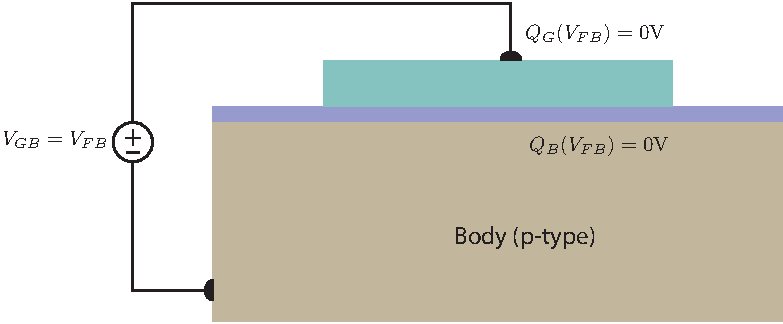
\includegraphics[width=.85\columnwidth]{mos_cap_flatband}
\caption{The flat-band voltage is defined as the gate-to-body voltage that results in net zero charge and zero fields in the MOS-C structure.}
\label{fig:mos_flatband}
\end{figure}
%%%%%%%%%%%%%%%%%%%%%%%%%%%%%%%%%%%%%%%%%%%%
\newpage
%%%%%%%%%%%%%%%%%%%%%%%%%%%%%%%%%%%%%%%%%%%%
%                 FIGURE                   %
%%%%%%%%%%%%%%%%%%%%%%%%%%%%%%%%%%%%%%%%%%%%
\begin{figure}[t]
\centering
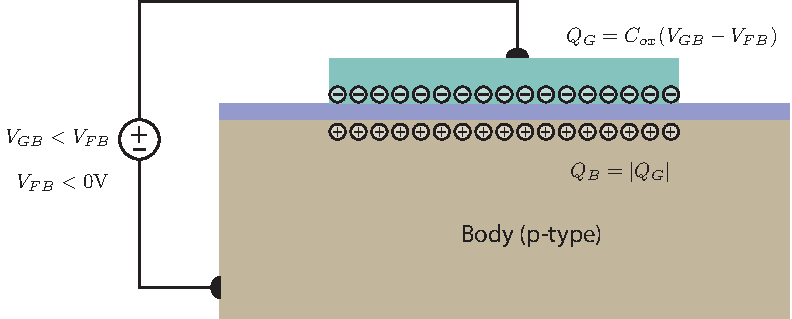
\includegraphics[width=.95\columnwidth]{mos_cap_acc}
\caption{In accumulation, a gate-to-body ($V_{GB}$) voltage less that the flat-band voltage is applied ($V_{FB}$), resulting in the accumulation of holes at the surface of the semiconductor, which terminate the fields in the oxide that originate from electrons in the gate.}
\label{fig:mos_accum}
\end{figure}
%%%%%%%%%%%%%%%%%%%%%%%%%%%%%%%%%%%%%%%%%%%%
%             SUBSECTION 7.3.3             %
%%%%%%%%%%%%%%%%%%%%%%%%%%%%%%%%%%%%%%%%%%%%
\subsection{Accumulation\texorpdfstring{$,\;V_{GB}<V_{FB}$}{}}
If we further decrease the potential beyond the “flat-band” condition, we essentially have a parallel plate capacitor, as shown in \emph{Fig.~\ref{fig:mos_accum}}.  Plenty of holes and electrons are available to charge up the plates, because we are making the gate more negative than the body.  So negative charges (electrons) flow into the gate, and holes can flow to, or \textbf{accumulate}\index{MOS capacitor!Regions of operation!accumulation} on, the surface of the device.  The negative bias (strong fields from the oxide) attracts the holes to reside under gate.
%%%%%%%%%%%%%%%%%%%%%%%%%%%%%%%%%%%%%%%%%%%%
%             SUBSECTION 7.3.4             %
%%%%%%%%%%%%%%%%%%%%%%%%%%%%%%%%%%%%%%%%%%%%
\subsection{Depletion\texorpdfstring{$,\;V_{GB}>V_{FB}$}{}}
In the \textbf{depletion}\index{MOS capacitor!Regions of operation!depletion} regime, shown in \emph{Fig.~\ref{fig:mos_dep}}, the situation is similar to equilibrium.  Since the potential in the gate is higher than the body, the body charge is made up of the depletion region (ionized group-III dopants for the $P$-type body), and there is a potential drop across the body and depletion region.  One way to understand this equilibrium scenario is to imagine what happens as the source voltage is increased beyond the flat-band condition.  At flat-band, by definition, there is no net charge in the gate or body.  As we apply a small voltage, positive charges enter the gate (electrons leave the gate), and negative charges (electrons) enter the body. Since the body is $P$-type, with the majority carriers being holes, most of these electrons will quickly recombine.  
%%%%%%%%%%%%%%%%%%%%%%%%%%%%%%%%%%%%%%%%%%%%
%                 FIGURE                   %
%%%%%%%%%%%%%%%%%%%%%%%%%%%%%%%%%%%%%%%%%%%%
\begin{figure}[H]
\centering
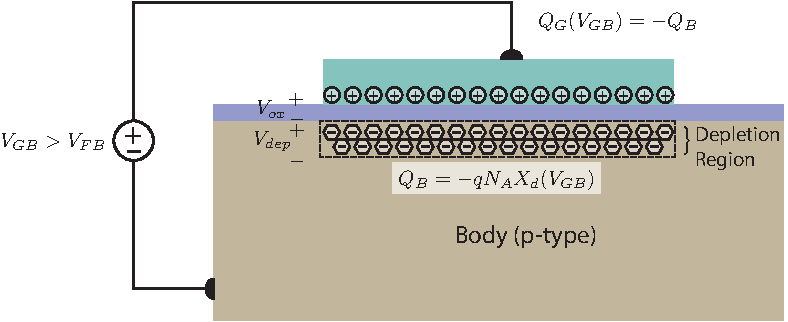
\includegraphics[width=.95\columnwidth]{mos_cap_depletion}
\caption{In depletion region, a gate-to-body ($V_{GB}$) voltage greater that the flat-band voltage is applied ($V_{FB}$).  The voltage should not be too large (less than inversion, defined below).  In this region, the oxide fields terminate on ionized dopant atoms.}
\label{fig:mos_dep}
\end{figure}
%%%%%%%%%%%%%%%%%%%%%%%%%%%%%%%%%%%%%%%%%%%%
\newpage
Recall that electric fields diverge (terminate) on charges.  Since there is a net positive charge in the gate, we have electric field lines that flow through the oxide and penetrate the silicon.  This non-zero body field will move holes away from the surface through the action of drift current.  This process will continue as long as field lines penetrate the body.  Notice that as holes are repelled from the surface, a net negative charge emerges due to the depletion region.  The action of the depletion region is to reduce the field strength, because some of the field lines terminate on the ionized dopants.  Eventually, the surface will be completely depleted of positive charge, and all the fields will terminate on ionized dopants.  Since the ionized dopants cannot move, not all the fields will terminate at the surface, but rather throughout the depletion region.
%%%%%%%%%%%%%%%%%%%%%%%%%%%%%%%%%%%%%%%%%%%%
%             SUBSECTION 7.3.5             %
%%%%%%%%%%%%%%%%%%%%%%%%%%%%%%%%%%%%%%%%%%%%
\subsection{Inversion\texorpdfstring{,\;$V_{GB}=V_T$}{}}
In the \textbf{inversion}\index{MOS capacitor!Regions of operation!inversion} regime, shown in \emph{Fig.~\ref{fig:mos_inv}}, as we further increase the gate voltage, because not all the charge resides at the surface, there is a larger and larger voltage drop across the depletion region.  In other words, the gate is "pulling" the surface of the body to a higher potential.  A higher surface potential makes it more favorable for electrons to stick around at the surface.  Recall that thermal \textbf{generation}\index{Generation} continually creates electron-hole pairs, and the steady-state number of electron/holes is regulated by \textbf{recombination}\index{Recombination}.  At the surface of the depletion region, electron-hole pair generation creates a situation that favors electrons because the holes are repelled from the surface and the electrons are attracted to the surface.  Eventually the surface potential increases to a point where the electron density at the surface equals the background ion density:
    \begin{align}
        n_s &= n_i\,e^{(q\,\phi_s/kT)} = N_A &\textit{Electron density at surface}\\[0.25cm]
        \phi_s &= -\phi_p
    \end{align}
At this point, the depletion region stops growing (effectively) and the extra charge is provided by the inversion charge at surface.  “Inversion” meaning that the surface is effectively $N$-type, even though it started as a $P$-type material.  
%%%%%%%%%%%%%%%%%%%%%%%%%%%%%%%%%%%%%%%%%%%%
%                 FIGURE                   %
%%%%%%%%%%%%%%%%%%%%%%%%%%%%%%%%%%%%%%%%%%%%
\begin{figure}[H]
\centering
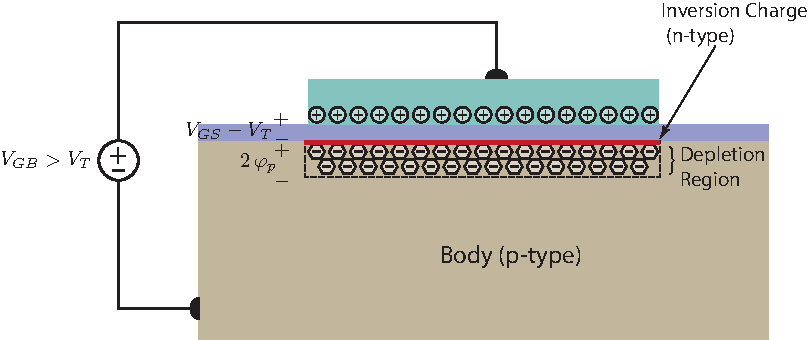
\includegraphics[width=\columnwidth]{mos_cap_inversion}
\caption{Inversion is defined as the gate-to-body ($V_{GB}$) voltage sufficient to invert the surface of the semiconductor from $P$-type to $N$-type, causing a sheet charge of electrons to accumulate at the surface.}
\label{fig:mos_inv}
\end{figure}
%%%%%%%%%%%%%%%%%%%%%%%%%%%%%%%%%%%%%%%%%%%%
\newpage
%%%%%%%%%%%%%%%%%%%%%%%%%%%%%%%%%%%%%%%%%%%%
%                 FIGURE                   %
%%%%%%%%%%%%%%%%%%%%%%%%%%%%%%%%%%%%%%%%%%%%
\begin{figure}[t]
\centering
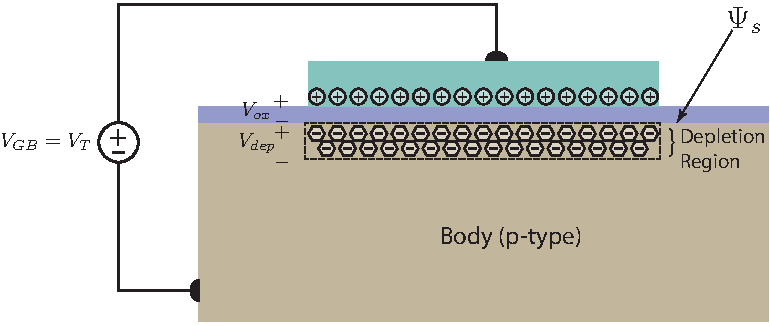
\includegraphics[width=.95\columnwidth]{mos_cap_threshold}
\caption{To derive the threshold voltage, it is important to realize that the gate-to-body voltage is dropped across both the oxide and the depletion region.  In absence of significant inversion charge at the surface, the total gate charge is compensated for entirely by depletion charge.}
\label{fig:mos_vt_derive}
\end{figure} 
%%%%%%%%%%%%%%%%%%%%%%%%%%%%%%%%%%%%%%%%%%%%%%%%%%%%%%%%%%%%%%%%%%%%%%%%%%%%%%%%%%%%%%%%
%%%%%%%%%%%%%%%%%%%%%%%%%%%%%%%%%%%%%%%%%%%%%%%%%%%%%%%%%%%%%%%%%%%%%%%%%%%%%%%%%%%%%%%%
%                                   SECTION 7.4                                        %
%%%%%%%%%%%%%%%%%%%%%%%%%%%%%%%%%%%%%%%%%%%%%%%%%%%%%%%%%%%%%%%%%%%%%%%%%%%%%%%%%%%%%%%%
%%%%%%%%%%%%%%%%%%%%%%%%%%%%%%%%%%%%%%%%%%%%%%%%%%%%%%%%%%%%%%%%%%%%%%%%%%%%%%%%%%%%%%%%
\section{MOS Device Threshold Voltage}
%%%%%%%%%%%%%%%%%%%%%%%%%%%%%%%%%%%%%%%%%%%%
%             SUBSECTION 7.4.1             %
%%%%%%%%%%%%%%%%%%%%%%%%%%%%%%%%%%%%%%%%%%%%
\subsection{Threshold Voltage Definition}
The \textbf{threshold voltage}\index{MOS capacitor!threshold voltage} is defined as the gate-body voltage that causes the surface to change from $P$-type to $N$-type.  For this condition, the \textbf{surface potential}\index{MOS capacitor!surface potential} has to equal the negative of the $P$-type potential.  We will show step-by-step that this voltage is equal to:
    \begin{align}
        \Aboxed{ V_{T_n} &= V_{FB} - 2\phi_p + \frac{1}{C_{ox}} \sqrt{2\,q\,\varepsilon _s\,N_A\,(-2\phi_p)} } &\textit{Threshold voltage, NMOS-C}
    \end{align}
%%%%%%%%%%%%%%%%%%%%%%%%%%%%%%%%%%%%%%%%%%%%
%             SUBSECTION 7.4.2             %
%%%%%%%%%%%%%%%%%%%%%%%%%%%%%%%%%%%%%%%%%%%%
\subsection{Derivation of \texorpdfstring{$V_T$}{Threshold Voltage}}
As shown in \emph{Fig.~\ref{fig:mos_vt_derive}}, the gate-to-body voltage is dropped across the oxide and the depletion region:
    \begin{equation*}
        V_{GB} = V_{ox} + V_{dep}
    \end{equation*}
To see this, do a KVL loop around the structure when a voltage source is added.  Recall from \emph{Fig.~\ref{fig:mos_cap_gate_body_short_gate}} that the built-in voltage cancels out around the loop since it appears twice with opposite polarity.  To cause inversion, we increase the gate voltage until the surface potential becomes sufficiently positive relative to the bulk.  Once we have reached the inversion regime the electron density is the same as the body hole density.  This means that compared to the bulk, the potential at the surface is at $-2\phi_p$.  This voltage is dropped across the depletion region:
    \begin{equation*}
        V_{dep} = -2 \phi_p
    \end{equation*}
If we apply a gate-to-body voltage of $V_{FB}$, then we know the fields and charge go to zero. This is a good starting point.  Next, the oxide voltage is calculated from the gate/bulk charge.  At the edge of inversion, the total bulk charge for inversion is given by:
    \begin{equation*}
        Q_{dep} = \sqrt{2 q \epsilon_s N_A (-2 \phi_p) }
    \end{equation*}
This means the voltage drop across the oxide is given by
    \begin{equation*}
        V_{ox} = Q_{dep} / C_{ox} 
    \end{equation*}
Putting this all together, we have:
    \begin{align*}
        V_{GB} = V_T &= V_{FB} + Q_{dep}/C_{ox} - 2 \phi_p\\[0.3cm]
        &= V_{FB} - 2 \phi_p + Q_{dep}/C_{ox}\\[0.1cm]
        &= V_{FB} - 2 \phi_p + \frac{1}{C_{ox}} \sqrt{2\,q\,\varepsilon _s\,N_A\,(-2\phi_p)}
    \end{align*}
Notice that we made some simplifying assumptions to arrive here.  We assumed zero inversion charge to reach this point, which of course is not quite correct.  However, it is a good approximation because the total inversion charge is still quite low, even if the density is high at the surface.  We also made the standard depletion approximation, and assumed that the surface depletion region is fully depleted.  This follows from the same arguments that we made when deriving the depletion region for the $PN$-junction.
%%%%%%%%%%%%%%%%%%%%%%%%%%%%%%%%%%%%%%%%%%%%%%%%%%%%%%%%%%%%%%%%%%%%%%%%%%%%%%%%%%%%%%%%
%%%%%%%%%%%%%%%%%%%%%%%%%%%%%%%%%%%%%%%%%%%%%%%%%%%%%%%%%%%%%%%%%%%%%%%%%%%%%%%%%%%%%%%%
%                                   SECTION 7.5                                        %
%%%%%%%%%%%%%%%%%%%%%%%%%%%%%%%%%%%%%%%%%%%%%%%%%%%%%%%%%%%%%%%%%%%%%%%%%%%%%%%%%%%%%%%%
%%%%%%%%%%%%%%%%%%%%%%%%%%%%%%%%%%%%%%%%%%%%%%%%%%%%%%%%%%%%%%%%%%%%%%%%%%%%%%%%%%%%%%%%
\section{Fields and Potential in Oxide/Substrate}
%%%%%%%%%%%%%%%%%%%%%%%%%%%%%%%%%%%%%%%%%%%%
%             SUBSECTION 7.5.1             %
%%%%%%%%%%%%%%%%%%%%%%%%%%%%%%%%%%%%%%%%%%%%
\subsection{Fields in oxide/substrate}
The electric field in the MOS-C structure is shown schematically and graphically in \emph{Fig.~\ref{fig:mos_field_oxide_semi}}.  Notice that the field in the oxide is constant, because the oxide is a good insulator and there are no charges in the oxide.  The oxide does exert itself through the permittivity, and because silicon has a dielectric constant that is about three times higher, the fields experience a discontinuity crossing the oxide/body boundary.  Also, the fields do not drop to zero in the body instantly because the body charges are distributed throughout the depletion region.  Under the assumption of uniform doping, the fields drop linearly until they return to zero at the edge of the depletion region.   
%%%%%%%%%%%%%%%%%%%%%%%%%%%%%%%%%%%%%%%%%%%%
%                 FIGURE                   %
%%%%%%%%%%%%%%%%%%%%%%%%%%%%%%%%%%%%%%%%%%%%
\begin{figure}[H]
\centering
\begin{tabular}{cc}
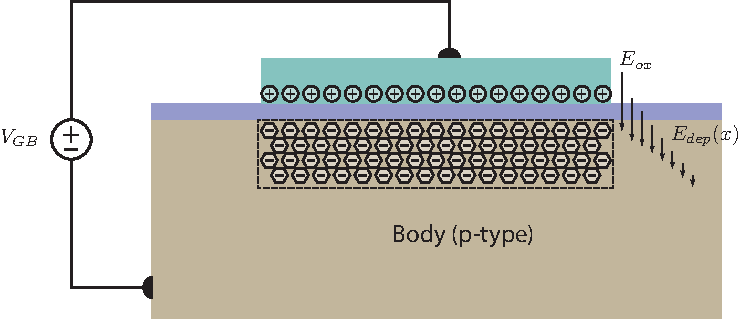
\includegraphics[width=.61\columnwidth]{mos_cap_Efields}\\
(a)\\
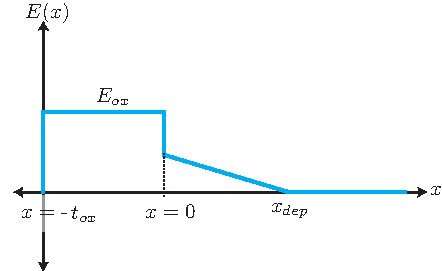
\includegraphics[width=.51\columnwidth]{MOS_E_field}\\
(b)\\
\end{tabular}
\caption{The electric field inside the oxide and transistor body shown (a) schematically, and (b) graphed as a function of $x$.  The discontinuity in the electric field is due to the difference in dielectric permittivity between $SiO_2$ and $Si$.  The linear variation in the depletion region is due to the uniform doping concentration of acceptor atoms.}
\label{fig:mos_field_oxide_semi}
\end{figure}
%%%%%%%%%%%%%%%%%%%%%%%%%%%%%%%%%%%%%%%%%%%%
\newpage
%%%%%%%%%%%%%%%%%%%%%%%%%%%%%%%%%%%%%%%%%%%%
%                 FIGURE                   %
%%%%%%%%%%%%%%%%%%%%%%%%%%%%%%%%%%%%%%%%%%%%
\begin{figure}[t]
\centering
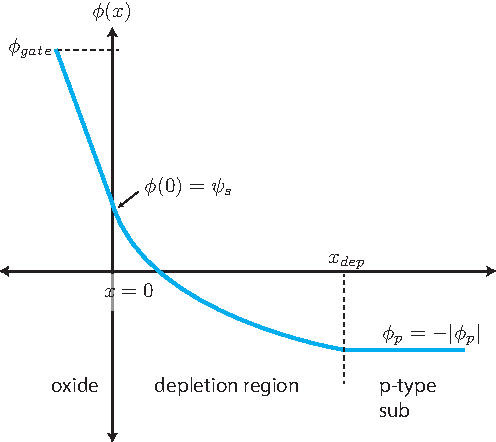
\includegraphics[width=.85\columnwidth]{MOS_potential}
\caption{The variation of electric potential through the oxide and depletion region.} \label{fig:MOS_potential}
\end{figure}
%%%%%%%%%%%%%%%%%%%%%%%%%%%%%%%%%%%%%%%%%%%%
%             SUBSECTION 7.5.2             %
%%%%%%%%%%%%%%%%%%%%%%%%%%%%%%%%%%%%%%%%%%%%
\subsection{Potential Variations in Oxide/Substrate}
The variation of the potential, the integral of the fields in \emph{Fig.~\ref{fig:mos_field_oxide_semi}}, is shown in \emph{Fig.~\ref{fig:MOS_potential}}.  The potential transitions smoothly across the oxide into the body.  The potential varies linearly in the oxide, and then quadratically in the body.  From this figure it is clear that pulling the gate voltage high pulls the surface potential to a value above the $P$-type region potential, thereby eventually transforming it from $P$-type to $N$-type. 
%%%%%%%%%%%%%%%%%%%%%%%%%%%%%%%%%%%%%%%%%%%%
%                 FIGURE                   %
%%%%%%%%%%%%%%%%%%%%%%%%%%%%%%%%%%%%%%%%%%%%
\begin{figure}[H]
\centering
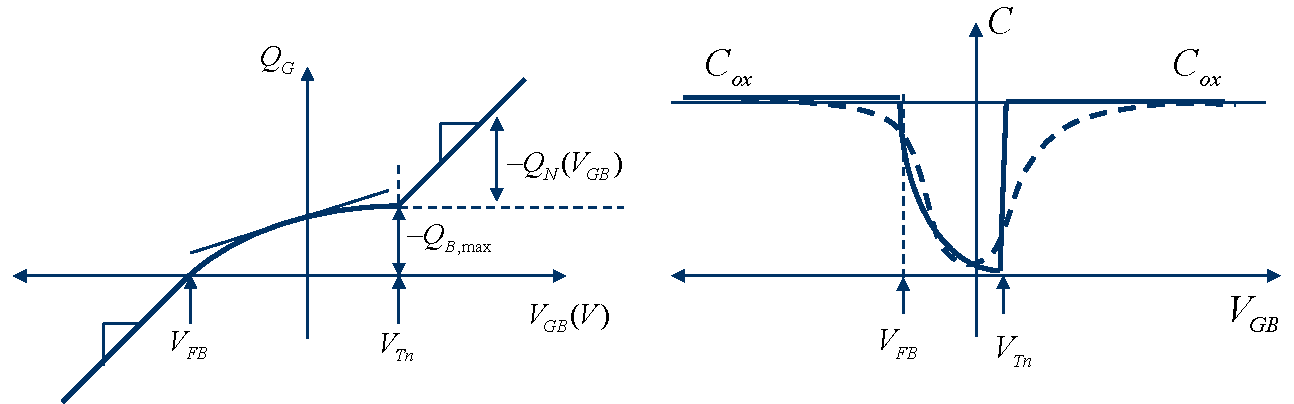
\includegraphics[width=\columnwidth]{mos_qv_cv}
\caption{The plot of charge vs. voltage $Q$-$V$ and small-signal capacitance vs. voltage $C$-$V$ for an MOS-C structure.  The breakpoints occur at the flat-band voltage $V_{FB}$ and the threshold voltage $V_T$.  The dashed line in the $C$-$V$ curve represents a more physical change in capacitance due to higher-order effects not discussed in this chapter.}
\label{fig:mos_qv_cv}
\end{figure}
%%%%%%%%%%%%%%%%%%%%%%%%%%%%%%%%%%%%%%%%%%%%
\newpage
%%%%%%%%%%%%%%%%%%%%%%%%%%%%%%%%%%%%%%%%%%%%%%%%%%%%%%%%%%%%%%%%%%%%%%%%%%%%%%%%%%%%%%%%
%%%%%%%%%%%%%%%%%%%%%%%%%%%%%%%%%%%%%%%%%%%%%%%%%%%%%%%%%%%%%%%%%%%%%%%%%%%%%%%%%%%%%%%%
%                                   SECTION 7.6                                        %
%%%%%%%%%%%%%%%%%%%%%%%%%%%%%%%%%%%%%%%%%%%%%%%%%%%%%%%%%%%%%%%%%%%%%%%%%%%%%%%%%%%%%%%%
%%%%%%%%%%%%%%%%%%%%%%%%%%%%%%%%%%%%%%%%%%%%%%%%%%%%%%%%%%%%%%%%%%%%%%%%%%%%%%%%%%%%%%%%
\section{Charge-Voltage (\texorpdfstring{$Q$-$V$}{Q-V}) and Capacitance-Voltage (\texorpdfstring{$C$-$V$}{C-V}) Curves}
%%%%%%%%%%%%%%%%%%%%%%%%%%%%%%%%%%%%%%%%%%%%
%             SUBSECTION 7.6.1             %
%%%%%%%%%%%%%%%%%%%%%%%%%%%%%%%%%%%%%%%%%%%%
\subsection{\texorpdfstring{$Q$-$V$}{Q-V} Curve for MOS Capacitor}
A plot of the charge versus voltage ($Q$-$V$) is shown in \emph{Fig.~\ref{fig:mos_qv_cv}}.  The charge is not a linear function of voltage, and so the capacitance curve ($C$-$V$), shown in the same figure, is really the small-signal capacitance\index{Small-signal capacitance}, which is the derivative of the $Q$-$V$ relation.  In accumulation, the charge is simply proportional to the applied gate-body bias, because the body acts like a second gate.  In inversion, the same is true because the surface of the structure is a charge sheet that terminates all additional field lines.  Notice that this curve is only valid under \textbf{quasi-static}\index{Quasi-static} conditions.  In other words, we have to allow enough time for thermal generation\index{Thermal generation} to supply electrons to the surface.  If a rapid voltage (like a step transition) is applied, there is insufficient time for generation and the response would have to come from the depletion region temporarily until sufficient time elapses for surface electron density to build up.  

The most complicated part of this curve is the depletion region.  The charge grows slower than linear since the voltage is applied over a depletion region, rather than just through the oxide.  
%%%%%%%%%%%%%%%%%%%%%%%%%%%%%%%%%%%%%%%%%%%%
%             SUBSECTION 7.6.2             %
%%%%%%%%%%%%%%%%%%%%%%%%%%%%%%%%%%%%%%%%%%%%
\subsection{MOS \texorpdfstring{$C$-$V$}{C-V} Curve}
Since the small-signal capacitance is slope of Q-V curve, it is not very difficult to see how the curve shown in the second part of \emph{Fig.~\ref{fig:mos_qv_cv}} arises.  The capacitance is constant in accumulation and inversion because in these regions the device is acting like a simple parallel plate capacitor.  The capacitance in the depletion region is smallest because the voltage drop occurs both across the oxide and across the depletion region.  The capacitance is non-linear in the depletion region.  
%%%%%%%%%%%%%%%%%%%%%%%%%%%%%%%%%%%%%%%%%%%%
%             SUBSECTION 7.6.3             %
%%%%%%%%%%%%%%%%%%%%%%%%%%%%%%%%%%%%%%%%%%%%
\subsection{\texorpdfstring{$C$-$V$}{C-V} Curve Equivalent Circuits}
%%%%%%%%%%%%%%%%%%%%%%%%%%%%%%%%%%%%%%%%%%%%
%                 FIGURE                   %
%%%%%%%%%%%%%%%%%%%%%%%%%%%%%%%%%%%%%%%%%%%%
\begin{figure}[tbh]
\centering
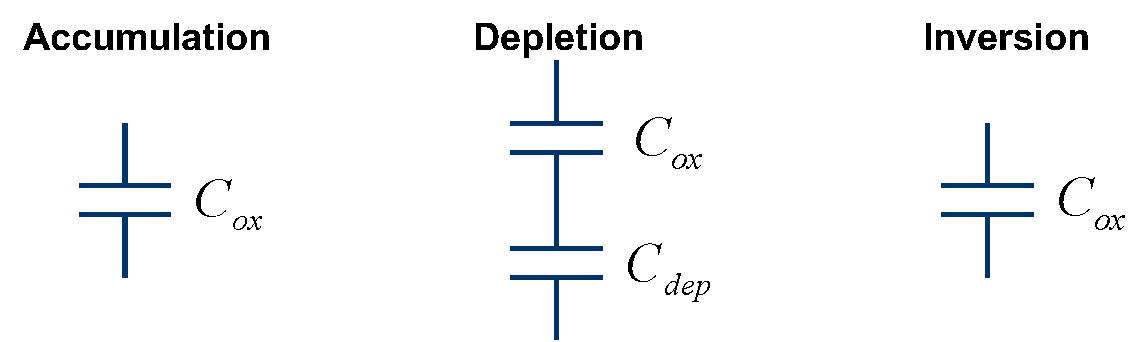
\includegraphics[width=\columnwidth]{mos_cv_circuits}
\caption{The equivalent circuit for a MOS-C capacitor for small-signal perturbations about a fixed operating point in accumulation, depletion, and inversion.}
\label{fig:mos_cv_circuits}
\end{figure}
%%%%%%%%%%%%%%%%%%%%%%%%%%%%%%%%%%%%%%%%%%%%
Equivalent small-signal circuits for the MOS-C are summarized in \emph{Fig.~\ref{fig:mos_cv_circuits}}.  In accumulation mode, the capacitance is just due to the voltage drop across $t_{ox}$, and we can calculate this capacitance per unit area from the parallel plate formula:
    \begin{align}
        \Aboxed{ C_{acc} &= C_{inv} = C_{ox} = \frac{\epsilon_{ox}}{t_{ox}} } &\textit{Capacitance, accumulation and inversion regime}
    \end{align}
The equivalent circuit applies in inversion.  Let's pause and discuss this in a bit more detail.  We are talking about \emph{small-signal} or incremental charges, not total charge.  So if the MOS-C is biased in accumulation, and an incremental voltage is applied to the device, the additional charges flow into the surface of the body and gate, and $C_{ox}$ is the relation between incremental charge and voltage.

In inversion, there is already a depletion region, but we are assuming that when an incremental voltage is applied that the depletion region does not grow.  Thus, all additional charges will flow to the surface of the device in the form of the inversion layer. This is why the small-signal equivalent circuit in inversion does not have anything about depletion in it.  Anything that is "frozen" in place has no impact on the small-signal response.

In the depletion region, the voltage drop is across the oxide and the depletion region.  Let's define the depletion region capacitance as follows:
    \begin{align}
        \Aboxed{ C_{dep} &= \frac{\varepsilon_s}{x_{dep}} } &\textit{Capacitance, depletion regime}
    \end{align}
Then we can say that in the depletion region, the gate-body incremental voltage "sees" two capacitors in series, as shown in the equivalent circuit:
    \begin{align}
        C_{tot} &= \frac{C_{dep}\,C_{ox}}{C_{dep} + C_{ox}} = \frac{C_{ox}}{1 + \frac{C_{dep}}{C_{ox}}}\\
        &= \frac{C_{ox}} {1 + \frac{\varepsilon_s}{\varepsilon_{ox}\frac{t_{ox}}{x_{dep}}}} &\textit{Total series capacitance in depletion regime}
    \end{align}
Since $x_{dep}$ depends on bias, we evaluate $x_{dep}$ at the value of the operating point of the circuit.  
%%%%%%%%%%%%%%%%%%%%%%%%%%%%%%%%%%%%%%%%%%%%
%             SUBSECTION 7.6.4             %
%%%%%%%%%%%%%%%%%%%%%%%%%%%%%%%%%%%%%%%%%%%%
\subsection{Numerical Example}
Let's work through the numbers to get a feel for the MOS capacitor.  Assume that it is a $P$-type substrate with an oxide thickness of $t_{ox} = 20\,nm$, and a body doping concentration of $N_A = \SI{5e16}{\cm^{-3}}$.
This gives rise to an oxide capacitance of:
    \begin{equation*}
        C_{ox} = \frac{\varepsilon_{ox}}{t_{ox}}
        = \frac{\SI[per-mode = fraction]{3.45e-13}{\farad\per\cm}}{\SI{2e-6}{\cm}}
        \approx \boxed{ 172.5\,nF }
    \end{equation*}
With reference to \emph{Eq.~\ref{eq:p_body_pot}} we can find that:
    \begin{equation*}
        \phi_p = -\left( \frac{kT}{q} \right) \cdot \ln \left( \frac{N_A}{n_i} \right)
        = -(0.026\,V)\cdot \ln \left( \frac{\SI{5e16}{\cm^{-3}}}{\SI{1e10}{\cm^{-3}}} \right)
        \approx \boxed{ -401\,mV }
    \end{equation*}
Let's first calculate the flat-band voltage.  Because we do not have any information about the gate doping level, let's assume that it is \textbf{degeneratively doped}\index{Degenerative doping}, so the potential of the poly-$n^+$ gate is $550\,mV$:
    \begin{equation*}
        V_{FB} = -(\phi_{n^+} - \phi_p) = -\big(550\,mV -(-402\,mV)\big) = -(550\,mV + 401\,mV) = \boxed{ -0.952\,V }
    \end{equation*}
Next, let's calculate the threshold voltage:
    \begin{align*}
        V_{T_n} &= V_{FB} - 2\phi_p + \frac{1}{C_{ox}} \sqrt{ 2\,q\,\varepsilon_s\,N_A\,(-2\phi_p) }\\[0.5cm]
        &= -(0.952\,V) + \big((-2)(-0.401)\big) \\[0.15cm]
        &\qquad + \frac{\sqrt{ 2\,(\SI{1.602e-19}{\coulomb})(\SI[per-mode = fraction]{1.0359e-12}{\farad\per\cm})(\SI{5e16}{\cm^{-3}})\,-2(-0.401\,V) }} {\SI{1.725e-7}{\farad}}\\[0.5cm]
        &= -0.952\,V + 0.802\,V + 0.668\,V\\[0.25cm]
        \Aboxed{&\approx0.52\,V}
    \end{align*}
Now let's apply a gate-to-body voltage:
    \begin{equation*}
        V_{GB} = -2.5 < V_{FB}
    \end{equation*}
Since the device is in accumulation, the entire voltage drop is across the oxide, and the oxide fields are given by:
    \begin{align*}
        \mathcal{E}_{ox} &= \frac{V_{ox}}{t_{ox}} = \frac{V_{GB} + \phi_{n^+} - \phi_p}{t_{ox}}\\[0.35cm]
        &= \frac{(-2.5\,V + 0.55\,V -(-0.401)}{\SI{2e-6}{\cm}}\\[0.35cm]
        &= \frac{-1.549\,V}{\SI{2e-6}{\cm}}\\[0.35cm]
        \Aboxed{ &= \SI[per-mode = fraction]{-8e5}{\volt\per\cm} }
    \end{align*}
The charge in the substrate (body) consist of holes:
    \begin{align*}
        Q_B &= -C_{ox}(V_{GB} - V_{FB})\\[0.25cm]
        &= -(\SI{1.725e-7}{F})\cdot\left(-2.5\, -(-0.952\,V) \right)\\[0.25cm]
        &= -(\SI{1.725e-7}{F})\cdot(-1.548\,V)\\[0.25cm]
        \Aboxed{&\approx \SI[per-mode = fraction]{2.67e-7}{\coulomb\per\cm^2} }
    \end{align*}
